%% LyX 2.3.6.2 created this file.  For more info, see http://www.lyx.org/.
%% Do not edit unless you really know what you are doing.
\documentclass[sigconf,nonacm]{acmart}
\usepackage[utf8]{inputenc}
\setcounter{secnumdepth}{3}
\setcounter{tocdepth}{3}
\synctex=-1
\usepackage{array}
\usepackage{verbatim}
\usepackage{mathtools}
\usepackage{graphicx}
\ifx\hypersetup\undefined
  \AtBeginDocument{%
    \hypersetup{unicode=true}
  }
\else
  \hypersetup{unicode=true}
\fi

\makeatletter

%%%%%%%%%%%%%%%%%%%%%%%%%%%%%% LyX specific LaTeX commands.
%% Because html converters don't know tabularnewline
\providecommand{\tabularnewline}{\\}
\floatstyle{ruled}
\newfloat{algorithm}{tbp}{loa}
\providecommand{\algorithmname}{Algorithm}
\floatname{algorithm}{\protect\algorithmname}

%%%%%%%%%%%%%%%%%%%%%%%%%%%%%% User specified LaTeX commands.
\usepackage{pgfplots}
\usepackage{subcaption}
\usepackage{adjustbox}
\usepackage{url}
%\usepackage{minted}


\usepgfplotslibrary{groupplots,dateplot}
\usetikzlibrary{
    patterns,
    chains,
    backgrounds,
    calc,
    shadings,
    shapes.arrows,
    arrows,
    shapes.symbols,
    shadows,
    positioning,
    decorations.markings,
    backgrounds,
    arrows.meta,
    external
}
\usepackage{array}
\usepackage{algorithmicx,algpseudocode}
% declaration of the new block
\algblock{ParFor}{EndParFor}
% customising the new block
\algnewcommand\algorithmicparfor{\textbf{parfor}}
\algnewcommand\algorithmicpardo{\textbf{do}}
\algnewcommand\algorithmicendparfor{\textbf{end}}
\algrenewtext{ParFor}[1]{\algorithmicparfor\ #1\ \algorithmicpardo}
\algrenewtext{EndParFor}{\algorithmicendparfor}
\renewcommand{\algorithmicrequire}{\textbf{Input:}} 
\renewcommand{\algorithmicensure}{\textbf{Output:}}

\pgfplotsset{compat=newest}

\newcommand{\code}[1]{\texttt{#1}}

\newif\iffinal

\iffinal
  \newcommand{\maxx}[1]{}
  \newcommand{\ryan}[1]{}
  \newcommand{\todo}[1]{}
\else
  \newcommand{\maxx}[1]{{\textcolor{red}{ Max: #1 }}}
  \newcommand{\ryan}[1]{{\textcolor{magenta}{ Ryan: #1 }}}
  \newcommand{\todo}[1]{{\textcolor{blue}{ TODO: #1 }}}
\fi

\makeatother

\begin{document}
\title{Ultrafast focus detection using multi-scale histologic features}
\author{Maksim Levental}
\affiliation{\institution{University of Chicago}}
\author{Ryan Chard}
\affiliation{\institution{Argonne National Laboratory}}
\author{Gregg A. Wildenberg}
\affiliation{\institution{University of Chicago}}
\begin{abstract}
We present a fast out-of-focus detection algorithm for electron microscopy
images collected serially. Such images are collected for the purposes
of post-processing tasks such as montaging, alignment, and image segmentation.
Such an algorithm is necessitated by recent increases in collection
rates owing to advances in microscopy technology. Our technique, \textit{Multi-scale
Histologic Feature Detection}, adapts classical computer vision techniques
and is based on detecting various fine-grained histologic features.
We further exploit the inherent parallelism in the technique by employing
GPGPU primitives in order to accelerate characterization. Tests are
performed that demonstrate near-real-time detection of out-of-focus
conditions. \textless We also deploy to funcX something something\textgreater .
We discuss extensions that enable scaling out to support multi-beam
microscopes and integration with existing focus systems for purposes
of implementing auto-focus.
\end{abstract}
\maketitle

\section{Introduction}

\label{sec:intro}

\begin{comment}
Advancements in the automation of serial scanning electron microscopy
(SEM) impose a regime where thousands, if not tens of thousands, of
images can now be automatically collected by researchers. This puts
greater demand on conventional auto-focus algorithms for ensuring
each image is in focus, as an alternative to the user manually evaluating
each image by eye. Without such algorithms, critical bottlenecks are
created where the user is forced to reacquire individual, deficient
(out-of-focus), images and manually reinsert them into the sequence
of thousands of other images already acquired. This is an onerous
task which requires taking into account alignment and boundary overlap.
Furthermore, failure to quickly identify and reacquire deficient images
negatively impacts the accuracy of downstream, post-processing; for
example 2D montaging, 3D alignment, or automatic segmentation pipelines.
While many microscopes have builtin auto-focus algorithms, these often
fail to achieve acceptable accuracy due to intrinsic mediating factors
(e.g. stage drift) and extrinsic mediating factors (e.g. sample artifacts,
non-uniformity in the sample).
\end{comment}

A fundamental goal of neuroscience is to map the anatomical relationships
of the brain. Currently this is challenging because electron microscopy,
an imaging method traditionally limited to small images, is the only
imaging modality with sufficient resolution to directly visualize
the connections, or synapses, between neurons. Recently, automated
serial electron microscopy, broadly called \textit{connectomics},
has been developed. This technique is characterized by thousands,
if not tens of thousands, of individual images being automatically
acquired in series and then registered to produce a volumetric dataset.
Such datasets allow neuroscientists to follow the tortuous path neurons
take through the brain to connect with each other (hence the name
connectomics). However, many of the steps that comprise the collection
of such datasets for connectomics require manual inspection causing
significant slowdowns in the rate at which datasets can be acquired.
Such bottlenecks significantly impact the size of the datasets that
can be reasonably acquired and studied. Furthermore, advances in electron
microscopes have increased the rate that datasets can be acquired
(e.g. \textasciitilde 10 Tbs/24hr \citet{zeiss:multisem550}) . This
further underscores the need for automation (in order that end-to-end
high throughput is achieved). %
\begin{comment}
Thus, without high fidelity automation of the imaging pipeline, the
field of connectomics will fail to advance and realize its full potential. 
\end{comment}

Auto-focus technology is a critical component of many imaging systems;
from consumer cameras (for purposes of convenience) to industrial
inspection tools to scientific instrumentation \citep{1545017}. Such
technology is typically either \textit{active} or \textit{passive};
active methods exploit some auxiliary device or mechanism to measure
the distance of the optics from the scene, while passive methods analyze
the definition or sharpness of an image by virtue of a proxy measure
called a \textit{criterion function}. Many electron microscopes incorporate
auto-focus techniques that attempt to focus the microscope before
image acquisition. Despite such functionality, out-of-focus (OOF)
images still occur at high rates (between 1\% and 10\%), depending
on the quality of the tissue sections being imaged. Such error rates
prevent effective automation since a prerequisite of the downstream
operations are that the images collected all have high degree-of-focus
(DOF). Without properly focused images, all downstream computational
steps (e.g. 2D tile montaging, 3D alignment, automatic segmentation)
will fail.

Thus, we seek to further the aims of automation by ensuring that images
acquired by the electron microscope have high DOF. While seemingly
a small step in the process, focus detection is nevertheless an extremely
critical step. Consequently, because imaging sections requires loading
and unloading sets of \textasciitilde 100-200 sections at a time,
failure to manually detect an out of focus image in real time causes
significant delays. The affected sample sets need to be reloaded,
desired field of view must be reconfigured, and reaquired images need
to be reinserted into the image stack. All such remediation steps
are time and labor intensive.

Our proposed technique, \textit{Multi-scale Histologic Feature Detection}
(MHFD), involves a second pass over the collected image, after it
has been acquired, using a computer vision system to detect a failure
to successfully achieve high DOF. We use feature detection \citep{Lindeberg2004FeatureDW}
as a criterion function, reasoning that the quantity of features detected
is positively correlated with DOF. To this end, we develop a feature
detector based on scale-space representations of images (see section
\eqref{sec:Backround}) but optimized for latency (rather than for
accuracy). Our solution achieves low latency detection of the OOF
condition with high correlation (see section \eqref{sec:Evaluation}). 

Note that we explicitly aim to augment existing microscopy equipment
without the need for costly and complex retrofitting. This precludes
mere improvements to auto-focus systems as they are, in essence, proprietary
black boxes from the perspective of the end user of a commerical electron
microscope. 

This rest of this article is organized as follows: section~\eqref{sec:Backround}
quickly reviews backround on scale-space feature detectors, section
\eqref{sec:implementation} describes our focus detection method in
the abstract and particular optimizations made in order to achieve
near-real-time performance, section \eqref{sec:Evaluation} reports
results of evaluating our method on sequences of images collected
at varying focus depths, section \eqref{sec:Discussion} discuss those
results, and section \eqref{sec:related} discusses related work and
how our work is distinct therefrom.

\section{Scale-space representations\label{sec:Backround}}

We base our multi-scale histologic feature detection technique on
classical scale-space representations of signals and images. We give
a brief overview (see \citep{Lindeberg2004FeatureDW} for a more comprehensive
review). 

The fundamental principle of scale-space feature detection is that
natural images possess structureful features at multiple scales and
that features at a particular scale isolated from features at other
scales. Thus any image $I\left(x,y\right)$ can transformed into a
scale-space representation $L\left(x,y,t\right)$, where $L\left(x',y',t'\right)$
represents the pixel intensity\textit{}\footnote{Hence, scale-space since we consider the image along dimensions of
scale and space.} at pixel coordinates $\left(x',y'\right)$ and \textit{scale $t'$.}
How to produce the representation of the image at each scale is discussed
in the forth coming. More importantly, such a representation lends
itself readily to scale sensitive feature detection owing to the fact
that features at a particular scale are decoupled from features at
other scales, thereby eliminating confounding detections. Examples
of structureful features that can be detected and characterized using
scale-space representations include edges, corners, ridges, and so
called blobs (roughly circular regions of uniform intensity).

A scale-space representation at a particular scale is constructed
by convolution of the image with a filter that satisfies the constraints
of non-enhancement of local extrema, scale invariance and rotational
invariance (along with some others \citep{duits2004axioms}). One
such filter \citep{koenderink1984structure} is the symmetric, mean
zero, two dimensional, Gaussian filter 
\[
G\left(x,y,\sigma\right)\coloneqq\frac{1}{2\pi\sigma^{2}}e^{-\frac{x^{2}+y^{2}}{2\sigma^{2}}}
\]
Thus, define the scale-space representation $L(x,y,t)$ of an image
$I(x,y)$ to be the convolution of that image with a mean zero Gaussian
filter: 

\[
L\left(x,y,t\right)\coloneqq G\left(x,y,t\right)*I\left(x,y\right)
\]
where $t$ determines the scale. $L(x,y,t)$ has the interpretation
that image structures of scale smaller than $\sqrt{t^{2}}=t$ have
been removed due to blurring. This is due to the fact that the variance
of the Gaussian filter is $t^{2}$ and features of this scale are
therefore ``beneath the noise floor'' of the filter or, in effect,
suppressed by filtering procedure. A corollary is that features with
approximate length scale $t$ will have maximal response upon being
filtered by $G(x,y,t)$. That is to say, for a $t$ scale feature
at pixel coordinates $\left(x,y\right)$ and for scales $t'<t<t''$
we have

\[
L\left(x,y,t'\right)<L\left(x,y,t\right)<L\left(x,y,t''\right)
\]
This is due to the fact that for scales $t'<t$, small scale features
will dominate the response and for $t<t''$, as already mentioned,
the feature will have been suppressed. 

Note that the aforementioned presumes having identified the pixel
coordinates $\left(x,y\right)$ as the locus of the feature. Thus,
in order to detect features across scales and space, maximal responses
in spatial dimensions $\left(x,y\right)$ need to also be characterized.
For such characterization one generally employs standard calculus
in order to identify critical points of second order derivatives.
Hence, we can construct scale-sensitive feature detectors by considering
critical points of linear and non-linear combinations of spatial derivatives
$\partial_{x},\partial_{y}$ and derivatives in scale $\partial_{t}$.
For example the scale derivative of the Laplacian
\begin{equation}
\partial_{t}\nabla^{2}L\coloneqq\partial_{t}\left(\partial_{x}^{2}+\partial_{y}^{2}\right)L\label{eqn:blobdetector}
\end{equation}
effectively detects regions of uniform pixel intensity (i.e. blobs).

\section{Multi-scale Histologic Feature Detection\label{sec:implementation}}

\begin{figure}
\centering \begin{subfigure}[b]{0.5\textwidth} \centering 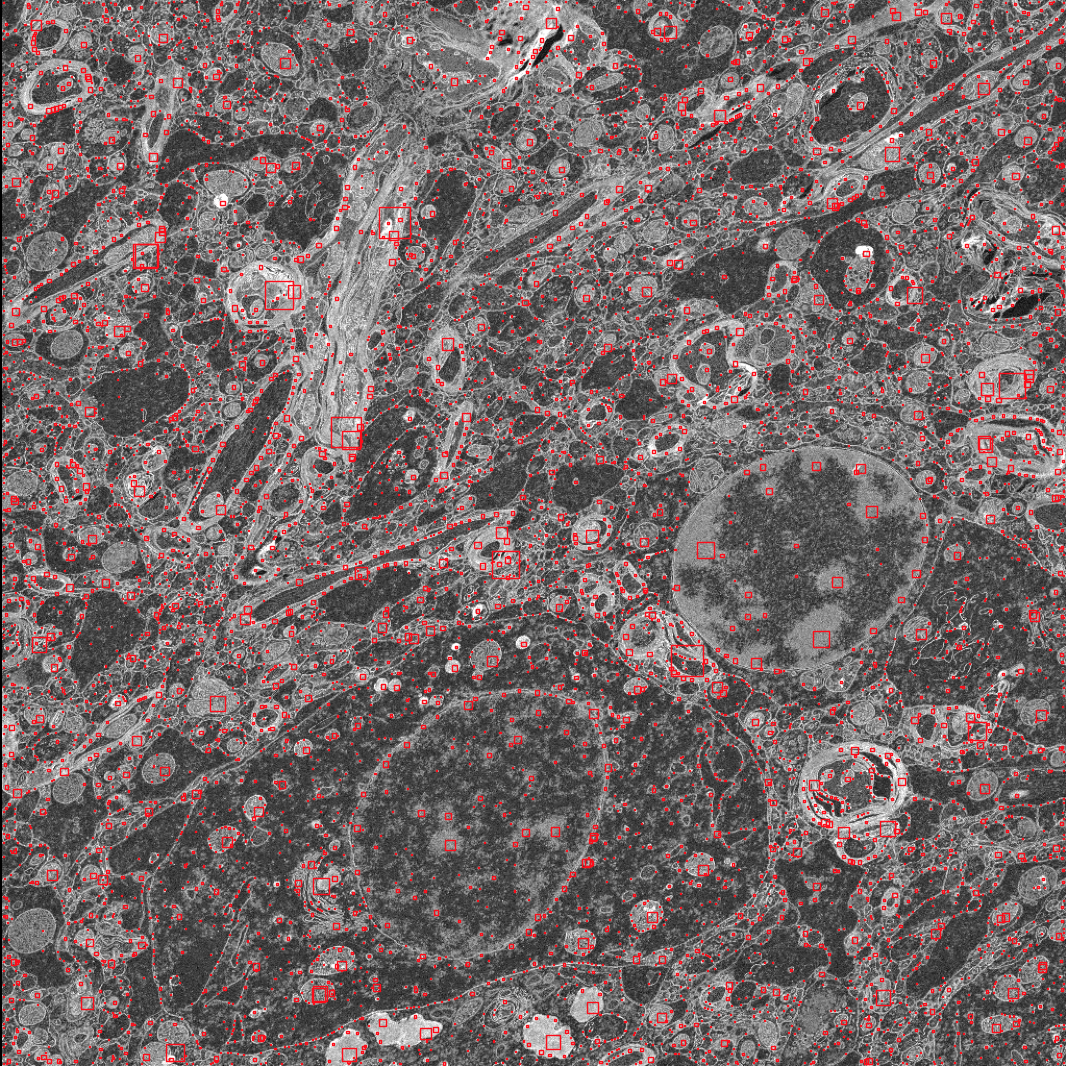
\includegraphics[width=1\linewidth]{in_focus}
\caption{Histologic features of an in-focus section.}
\label{subfig:infocus} \end{subfigure} 

\medskip{}
\begin{subfigure}[b]{0.5\textwidth} \centering 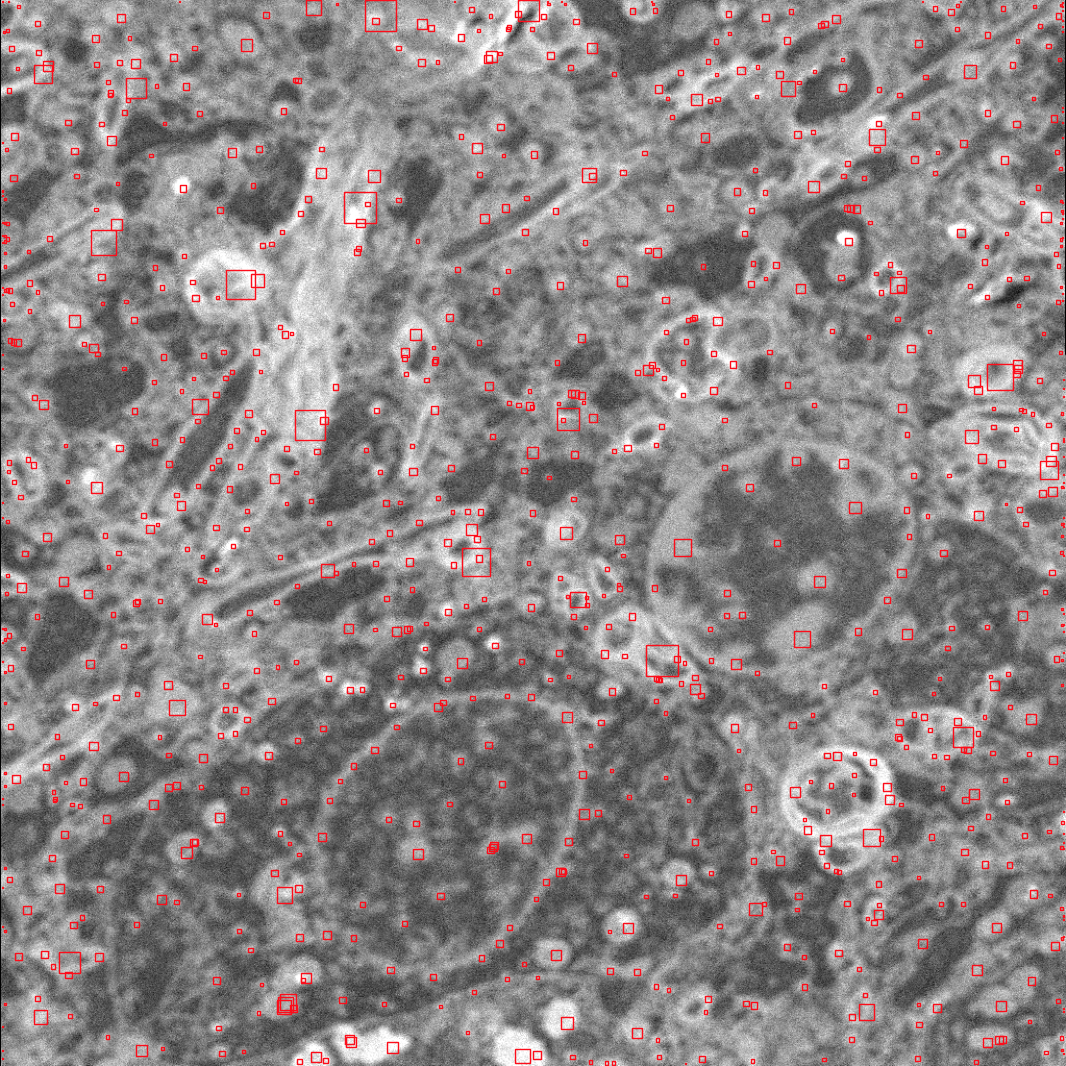
\includegraphics[width=1\linewidth]{out_of_focus}
\caption{Histologic features of an out-of-focus section.}
\label{subfig:outoffocus} \end{subfigure} \caption{Comparison of sections with histologic feature recognition as a function
of focal depth.}
\label{fig:histfeatsimages} 
\end{figure}

We propose to use histologic feature detection at multiple scales
as a criterion function, reasoning that the absolute quantity of features
detected at multiple scales is positively correlated with DOF (see
figure \eqref{fig:histfeatsimages}). For our particular use-case
this is tantamount to detecting histologic structures ranging from
cell walls to whole organelles. The key insight is that the ability
to resolve structure across the range of feature scales is highly
correlated with a high-definition image. To this end, we develop a
feature detector based on eqn. \eqref{eqn:blobdetector} but optimized
for latency (rather than for accuracy). 

Firstly, in order to verify our hypothesis that detecting features
across a range of scales is correlated with DOF, we compare the number
of histologic features detected as a function of absolute deviation
from in-focus ($\lvert f-f'\rvert$ where $f'$ is the correct focal
depth) for a series of sections with known focal depth (see figure
\eqref{subfig:degreeoofcurve}). We observe a very strong log-linear
relationship (see figure \eqref{subfig:degreeooffit}). Fitting a
log-linear relationship produces a line with $r=-0.9754$, confirming
our hypothesis that quantity of histologic features detected is a
good proxy measure for DOF. Note that the log-linear relationship
corresponds to a roughly quadratic decrease in the number of histologic
features detected. This is to be expected since, intuitively, a twice
improved DOF of a two dimensional image yields improved detection
along both spatial dimensions and thus a four times increased quantity
of histologic features detected.

\begin{figure}
\centering \begin{subfigure}[b]{0.5\textwidth} \centering % This file was created by tikzplotlib v0.9.8.
\begin{tikzpicture}[trim axis left,trim axis right]

\definecolor{color0}{rgb}{0.12156862745098,0.466666666666667,0.705882352941177}

\begin{axis}[
scaled y ticks=base 10:-3,
legend cell align={left},
legend style={fill opacity=0.8, draw opacity=1, text opacity=1, draw=white!80!black},
tick align=outside,
tick pos=left,
% title={Feature count vs. OOF},
x grid style={white!69.0196078431373!black},
xlabel={Degree of OOF},
xmin=-1.09892007559144e-06, xmax=2.31000189170211e-05,
xtick style={color=black},
xmajorgrids,
ymajorgrids,
y grid style={white!69.0196078431373!black},
ylabel={\# features},
ymin=99.9931235536055, ymax=9059.85673521721,
ytick style={color=black},
% y tick label style={/pgf/number format/sci}
]
\addplot [draw=color0, fill=color0, forget plot, mark=*, mark size=1, only marks, mark options={solid,fill opacity=0}]
table{%
x  y
2.89713740402389e-08 7023
1.79997717738205e-05 977
9.99997577071001e-06 1882
2.00011560321043e-06 6755
6.00014606118044e-06 4607
1.20001917481398e-05 2045
2.19998022317905e-05 743
1.99991485475958e-06 6791
3.99993008374979e-06 5606
5.99994531274e-06 3664
1.80000366866596e-05 899
2.00000519156498e-05 798
8.00016129016978e-06 3590
1.000017651916e-05 2672
1.400020697713e-05 1644
1.99997870028003e-05 874
7.99996054173021e-06 2513
1.40000062286896e-05 1233
1.60002222061202e-05 1185
1.19999909997002e-05 1419
1.60000214576702e-05 1056
4.00013083219977e-06 5610
2.20000671446296e-05 728
1.400020697713e-05 1172
3.99993008374979e-06 6308
7.99996054173021e-06 2688
9.99997577071001e-06 2037
1.03169680003984e-09 7000
1.000017651916e-05 1794
2.19998022317905e-05 741
1.99991485475958e-06 6987
5.99994531274e-06 4299
1.40000062286896e-05 1291
1.80000366866596e-05 988
2.00011560321043e-06 6389
4.00013083219977e-06 4785
6.00014606118044e-06 3080
8.00016129016978e-06 2329
1.20001917481398e-05 1472
1.60002222061202e-05 995
1.79997717738205e-05 882
1.19999909997002e-05 1595
1.60000214576702e-05 1103
2.00000519156498e-05 847
2.20000671446296e-05 781
1.99997870028003e-05 798
1.14187389609749e-07 8645
1.74120792746993e-06 8487
4.00013083219977e-06 5997
2.19998022317905e-05 831
1.99991485475958e-06 8516
3.99993008374979e-06 6280
9.99997577071001e-06 2037
1.80000366866596e-05 1004
6.00014606118044e-06 3510
8.00016129016978e-06 2658
1.20001917481398e-05 1517
1.60002222061202e-05 1095
7.99996054173021e-06 2740
2.00000519156498e-05 888
1.000017651916e-05 1958
1.79997717738205e-05 1022
1.99997870028003e-05 899
1.19999909997002e-05 1634
1.40000062286896e-05 1333
1.60000214576702e-05 1118
1.400020697713e-05 1253
5.99994531274e-06 3899
};
% \addplot [semithick, red]
% table {%
% 1.03169680003984e-09 8652.59020741432
% 2.89713740402389e-08 8621.47458132233
% 1.14187389609749e-07 8527.26131703851
% 1.74120792746993e-06 6913.51092038955
% 1.99991485475958e-06 6686.69355019204
% 1.99991485475958e-06 6686.69355019204
% 1.99991485475958e-06 6686.69355019204
% 2.00011560321043e-06 6686.52046851991
% 2.00011560321043e-06 6686.52046851991
% 3.99993008374979e-06 5166.70076818288
% 3.99993008374979e-06 5166.70076818288
% 3.99993008374979e-06 5166.70076818288
% 4.00013083219977e-06 5166.56703075379
% 4.00013083219977e-06 5166.56703075379
% 4.00013083219977e-06 5166.56703075379
% 5.99994531274e-06 3992.22674518632
% 5.99994531274e-06 3992.22674518632
% 5.99994531274e-06 3992.22674518632
% 6.00014606118044e-06 3992.1234084266
% 6.00014606118044e-06 3992.1234084266
% 6.00014606118044e-06 3992.1234084266
% 7.99996054173021e-06 3084.72952084398
% 7.99996054173021e-06 3084.72952084398
% 7.99996054173021e-06 3084.72952084398
% 8.00016129016978e-06 3084.6496741889
% 8.00016129016978e-06 3084.6496741889
% 8.00016129016978e-06 3084.6496741889
% 9.99997577071001e-06 2383.52098318378
% 9.99997577071001e-06 2383.52098318378
% 9.99997577071001e-06 2383.52098318378
% 1.000017651916e-05 2383.45928695194
% 1.000017651916e-05 2383.45928695194
% 1.000017651916e-05 2383.45928695194
% 1.19999909997002e-05 1841.70840227035
% 1.19999909997002e-05 1841.70840227035
% 1.19999909997002e-05 1841.70840227035
% 1.20001917481398e-05 1841.66073058486
% 1.20001917481398e-05 1841.66073058486
% 1.20001917481398e-05 1841.66073058486
% 1.40000062286896e-05 1423.05851843724
% 1.40000062286896e-05 1423.05851843724
% 1.40000062286896e-05 1423.05851843724
% 1.400020697713e-05 1423.02168329095
% 1.400020697713e-05 1423.02168329095
% 1.400020697713e-05 1423.02168329095
% 1.60000214576702e-05 1099.57447357174
% 1.60000214576702e-05 1099.57447357174
% 1.60000214576702e-05 1099.57447357174
% 1.60002222061202e-05 1099.54601164414
% 1.60002222061202e-05 1099.54601164414
% 1.60002222061202e-05 1099.54601164414
% 1.79997717738205e-05 849.652567006649
% 1.79997717738205e-05 849.652567006649
% 1.79997717738205e-05 849.652567006649
% 1.80000366866596e-05 849.623544825807
% 1.80000366866596e-05 849.623544825807
% 1.80000366866596e-05 849.623544825807
% 1.99997870028003e-05 656.512899491502
% 1.99997870028003e-05 656.512899491502
% 1.99997870028003e-05 656.512899491502
% 2.00000519156498e-05 656.490474517362
% 2.00000519156498e-05 656.490474517362
% 2.00000519156498e-05 656.490474517362
% 2.19998022317905e-05 507.276978773357
% 2.19998022317905e-05 507.276978773357
% 2.19998022317905e-05 507.276978773357
% 2.20000671446296e-05 507.259651356497
% 2.20000671446296e-05 507.259651356497
% };
% \addlegendentry{\#features $\approx 8653.74e^{-128941.61x}$}
\end{axis}

\end{tikzpicture}

\caption{Number of histologic features as a function of absolute deviation
from focused ($\lvert f-f'\rvert$ where $f'$ is the correct focal
depth).}
\label{subfig:degreeoofcurve} \end{subfigure} 

\medskip{}
\begin{subfigure}[b]{0.5\textwidth} \centering % This file was created by tikzplotlib v0.9.8.
\begin{tikzpicture}[trim axis left,trim axis right]

\definecolor{color0}{rgb}{0.12156862745098,0.466666666666667,0.705882352941177}

\begin{axis}[
legend cell align={left},
legend style={fill opacity=0.8, draw opacity=1, text opacity=1, draw=white!80!black},
tick align=outside,
tick pos=left,
% title={Log feature count vs. OOF},
x grid style={white!69.0196078431373!black},
xlabel={Degree of OOF},
xmin=-1.09892007559144e-06, xmax=2.31000189170211e-05,
xtick style={color=black},
y grid style={white!69.0196078431373!black},
ylabel={log (\#features)},
xmajorgrids,
ymajorgrids,
ymin=6.26154869922026, ymax=9.1982215266363,
ytick style={color=black}
]
\addplot [draw=color0, fill=color0, forget plot, mark=*, only marks]
table{%
x  y
2.89713740402389e-08 8.85694575615902
1.79997717738205e-05 6.88448665204278
9.99997577071001e-06 7.54009032014532
2.00011560321043e-06 8.8180382503943
6.00014606118044e-06 8.43533216493592
1.20001917481398e-05 7.6231530684769
2.19998022317905e-05 6.61069604471776
1.99991485475958e-06 8.82335348511379
3.99993008374979e-06 8.63159273172473
5.99994531274e-06 8.20631072579402
1.80000366866596e-05 6.80128303447162
2.00000519156498e-05 6.68210859744981
8.00016129016978e-06 8.18590748148232
1.000017651916e-05 7.89058253465654
1.400020697713e-05 7.40488757561612
1.99997870028003e-05 6.77308037565554
7.99996054173021e-06 7.82923253754359
1.40000062286896e-05 7.11720550316434
1.60002222061202e-05 7.07749805356923
1.19999909997002e-05 7.25770767716004
1.60000214576702e-05 6.96224346426621
4.00013083219977e-06 8.63230599851674
2.20000671446296e-05 6.59030104819669
1.400020697713e-05 7.06646697013696
3.99993008374979e-06 8.74957394808293
7.99996054173021e-06 7.89655270164304
9.99997577071001e-06 7.61923341622681
1.03169680003984e-09 8.85366542803745
1.000017651916e-05 7.49220304261874
2.19998022317905e-05 6.60800062529609
1.99991485475958e-06 8.85180655855245
5.99994531274e-06 8.36613771649628
1.40000062286896e-05 7.16317239084664
1.80000366866596e-05 6.89568269774787
2.00011560321043e-06 8.76233304060234
4.00013083219977e-06 8.47324130388705
6.00014606118044e-06 8.03268487596762
8.00016129016978e-06 7.75319426988434
1.20001917481398e-05 7.29437729928882
1.60002222061202e-05 6.90274273715859
1.79997717738205e-05 6.78219205600679
1.19999909997002e-05 7.37462901521894
1.60000214576702e-05 7.0057890192535
2.00000519156498e-05 6.74170069465205
2.20000671446296e-05 6.66057514983969
1.99997870028003e-05 6.68210859744981
1.14187389609749e-07 9.06473639811739
1.74120792746993e-06 9.04629085996968
4.00013083219977e-06 8.69901462316851
2.19998022317905e-05 6.72262979485545
1.99991485475958e-06 9.04970202601337
3.99993008374979e-06 8.74512525946224
9.99997577071001e-06 7.61923341622681
1.80000366866596e-05 6.91174730025167
6.00014606118044e-06 8.16337131645991
8.00016129016978e-06 7.88532923927319
1.20001917481398e-05 7.32448997934853
1.60002222061202e-05 6.9985096422506
7.99996054173021e-06 7.91571319938212
2.00000519156498e-05 6.78897174299217
1.000017651916e-05 7.57967882309046
1.79997717738205e-05 6.92951677076365
1.99997870028003e-05 6.80128303447162
1.19999909997002e-05 7.39878627541995
1.40000062286896e-05 7.19518732017871
1.60000214576702e-05 7.01929665371504
1.400020697713e-05 7.13329595489607
5.99994531274e-06 8.2684753889826
};
\addplot [semithick, red]
table {%
1.03169680003984e-09 8.94179754399353
2.89713740402389e-08 8.93856304962636
1.14187389609749e-07 8.92869784180801
1.74120792746993e-06 8.74034245317065
1.99991485475958e-06 8.71039271209553
1.99991485475958e-06 8.71039271209553
1.99991485475958e-06 8.71039271209553
2.00011560321043e-06 8.71036947203703
2.00011560321043e-06 8.71036947203703
3.99993008374979e-06 8.47885682365952
3.99993008374979e-06 8.47885682365952
3.99993008374979e-06 8.47885682365952
4.00013083219977e-06 8.47883358360112
4.00013083219977e-06 8.47883358360112
4.00013083219977e-06 8.47883358360112
5.99994531274e-06 8.24732093522351
5.99994531274e-06 8.24732093522351
5.99994531274e-06 8.24732093522351
6.00014606118044e-06 8.24729769516622
6.00014606118044e-06 8.24729769516622
6.00014606118044e-06 8.24729769516622
7.99996054173021e-06 8.01578504678751
7.99996054173021e-06 8.01578504678751
7.99996054173021e-06 8.01578504678751
8.00016129016978e-06 8.01576180673031
8.00016129016978e-06 8.01576180673031
8.00016129016978e-06 8.01576180673031
9.99997577071001e-06 7.7842491583527
9.99997577071001e-06 7.7842491583527
9.99997577071001e-06 7.7842491583527
1.000017651916e-05 7.78422591829431
1.000017651916e-05 7.78422591829431
1.000017651916e-05 7.78422591829431
1.19999909997002e-05 7.5527132699167
1.19999909997002e-05 7.5527132699167
1.19999909997002e-05 7.5527132699167
1.20001917481398e-05 7.5526900298595
1.20001917481398e-05 7.5526900298595
1.20001917481398e-05 7.5526900298595
1.40000062286896e-05 7.32117738148079
1.40000062286896e-05 7.32117738148079
1.40000062286896e-05 7.32117738148079
1.400020697713e-05 7.3211541414235
1.400020697713e-05 7.3211541414235
1.400020697713e-05 7.3211541414235
1.60000214576702e-05 7.08964149304589
1.60000214576702e-05 7.08964149304589
1.60000214576702e-05 7.08964149304589
1.60002222061202e-05 7.08961825298749
1.60002222061202e-05 7.08961825298749
1.60002222061202e-05 7.08961825298749
1.79997717738205e-05 6.85813627279123
1.79997717738205e-05 6.85813627279123
1.79997717738205e-05 6.85813627279123
1.80000366866596e-05 6.85810560460998
1.80000366866596e-05 6.85810560460998
1.80000366866596e-05 6.85810560460998
1.99997870028003e-05 6.62660038435643
1.99997870028003e-05 6.62660038435643
1.99997870028003e-05 6.62660038435643
2.00000519156498e-05 6.62656971617397
2.00000519156498e-05 6.62656971617397
2.00000519156498e-05 6.62656971617397
2.19998022317905e-05 6.39506449592042
2.19998022317905e-05 6.39506449592042
2.19998022317905e-05 6.39506449592042
2.20000671446296e-05 6.39503382773917
2.20000671446296e-05 6.39503382773917
};
\addlegendentry{log (\#features) $\approx -115767.06x + 8.94$}
\end{axis}

\end{tikzpicture}

\caption{Log plot and line fit with $r=-0.9754$.}
\label{subfig:degreeooffit} \end{subfigure} \caption{Comparison of histologic feature recognition as a function of focal
depth.}
\label{fig:histfeats} 
\end{figure}

We now discuss the design and implementation\footnote{\href{https://github.com/makslevental/cuda_blob/}{https://github.com/makslevental/cuda\_blob/}}
of our multi-scale histologic feature detector, with particular attention
paid to optimizations in consideration of inference latency. Eqn.
\eqref{eqn:blobdetector} permits a discretization\footnote{By virtue of $G$ being the Green's function of the heat equation
$t\nabla^{2}G=\partial_{t}G$.} called \textit{Difference of Gaussians} (DoG) (see~\citep{marr1980theory})
\[
t^{2}\nabla^{2}L\approx t\times\left(L\left(x,y,t+\delta t\right)-L\left(x,y,t\right)\right)
\]
Therefore, define 
\begin{itemize}
\item $n$, which determines the granularity of the scales detected 
\item $\min_{t}$, the minimum scale detected 
\item $\max_{t}$, the maximum scale detected 
\item $\delta t\coloneqq\left(\max_{t}-\min_{t}\right)/n$ 
\item $t_{i}\coloneqq\min_{t}+\left(i-1\right)\times\delta t$, the discrete
scales detected 
\end{itemize}
and finally the discretized DoG 
\begin{equation}
\operatorname{DoG}\left(x,y,i\right)\coloneqq t_{i}\times\left(L\left(x,y,t_{i+1}\right)-L\left(x,y,t_{i}\right)\right)\label{eqn:dog}
\end{equation}
This produces a sequence $\left\{ \operatorname{DoG}\left(x,y,i\right)\mid i=1,\dots,n\right\} $
of filtered and scaled images (called a Gaussian pyramid \citep{derpanis2005gaussian}).
Note that there are alternative convetions for how each difference
in the definition of $\operatorname{DoG}\left(x,y,i\right)$ should
be scaled (including partitioning into so called \textit{octaves}
\citep{1095851}) but we empirically determine that linear scaling
is sufficient for our needs.

Computing maxima of $\operatorname{DoG}\left(x,y,i\right)$ in the
scale dimension (equivalently critical points of eqn. \eqref{eqn:blobdetector})
necessarily entails computing local\footnote{In a small pixel neighborhood in both space and scale dimensions.}
maxima at every scale. We make the heuristic assumption that, in each
pixel neighborhood that corresponds to a feature, there is a single
unique and maximal response at some scale $t$. This response corresponds
to the scale at which the variance of the Gaussian filter $G$ most
closely corresponds to the scale of the feature (see section \eqref{sec:Backround}).
We therefore search for local maxima in spatial dimensions $x,y$
but global maxima in the scale dimension 
\begin{equation}
\left\{ \left(\hat{x}_{j},\hat{y}_{j},\hat{i}_{j}\right)\right\} \coloneqq\operatorname*{argmaxlocal}_{x,y}\operatorname*{argmax}_{i}\operatorname{DoG}\left(x,y,i\right)\label{eqn:argmax}
\end{equation}
where the subscript $j$ indexes over the features detected. Once
all such maxima are identified it suffices to compute and report the
cardinality of $\left\{ \left(\hat{x}_{j},\hat{y}_{j},\hat{i}_{j}\right)\right\} $
as criterion function value.

We now discuss practical (i.e. implementation) optimizations. It is
readily apparent that our histologic feature detector is parallelizable;
for each scale $t_{i}$ we can compute $L\left(x,y,t_{i}\right)$
independently of all other $L\left(x,y,t_{j}\right)$ (for $j\neq i$).
A further parallelization is possible for the $\operatorname*{argmax}$
operation, since the maxima are computed independently across distinct
neighborhoods of pixels. In order to maximally exploit this we first
perform the inner $\operatorname*{argmax}$ in eqn. \eqref{eqn:argmax}
on block of columns of $\left\{ \operatorname{DoG}\left(x,y,i\right)\right\} $
in parallel, thereby effectively reducing the Gaussian pyramid to
a single image. Note that when GPU memory is sufficient we can compute
the $\operatorname*{argmax}$ across all columns simulataneously (and
other wise within a constant number of steps). We then perform the
outer $\operatorname*{argmaxlocal}_{x,y}$ on disjoint pixel neighborhoods
of the flattened image in parallel as well. 

Note that the implementation of the inner $\operatorname*{argmax}$
is ``free'', since the $\operatorname*{argmax}$ primitive is implemented
in exactly this way in most GPGPU libraries \citep{CUB} and thus
our substitution of $\operatorname*{argmax}_{i}$ for $\operatorname*{argmaxlocal}_{i}$
yields a small but not insignificant latency decrease. The outer $\operatorname*{argmaxlocal}$
is implemented using a comparison against $\operatorname{MaxPool2D}(n,n)$
(with $n=3$) (see \citep{9307788} for details on this technique).
Employing $\operatorname{MaxPool2D}$ in this way has the added benefit
of effectively performing non-maximum suppression \citep{1699659},
since it effectively rejects spurrious candidate maxima within a $3\times3$
neighborhood of a true maximum.

Typically one would compute $L(x,y,t_{i})$ in the conventional way
(by linearly convolving $G$ and $I$) but prior work has shown \citep{9307788}
that performing the convolution in the Fourier domain is much more
efficient; namely 
\[
L\left(x,y,t_{i}\right)=\mathcal{F}^{-1}\big\{\mathcal{F}\left\{ G\left(x,y,t_{i}\right)\right\} \cdot\mathcal{F}\left\{ I\left(x,y\right)\right\} \big\}
\]
where $\mathcal{F}\left\{ \cdot\right\} ,\mathcal{F}^{-1}\left\{ \cdot\right\} $
are the Fourier transform and inverse Fourier transform, respectively.
This approach has the additional advantage that we can make use of
highly optimized Fast Fourier Transform (FFT) routines made available
by GPGPU libraries.

One remaining detail is histogram stretching of the images. Due to
the dynamic range (i.e. variable bit depth) of the microscope we need
to normalize the histogram of pixel values; we do this by saturating
$.175\%$ of the darkest pixels, saturating $.175\%$ of the lightest
pixels, and mapping the entire range to $[0,1]$. We find this gives
us consistently robust results with respect to noise and anomalous
features. This histogram normalization is also parallelized using
GPU primitives.

In summary our technique is presented in alg. \eqref{alg:Multi-scale-Histologic-Feature}.
\begin{algorithm}
\caption{Multi-scale Histologic Feature Detection\label{alg:Multi-scale-Histologic-Feature}}

\begin{algorithmic}[1]
\Require{$I\left(x,y\right), n, \min_{t}, \max_{t}, M$}
\State $I'\left(x,y\right) \coloneqq \texttt{HistorgramStretch}(I\left(x,y\right))$
\State \texttt{Broadcast}$\left(I'\left(x,y\right), M\right)$
\ParFor{$m \coloneqq 1,\dots, M$}
  \ParFor{$i\in I_{m}$}
    \State $L\left(x,y,t_{i}\right) \coloneqq \mathcal{F}^{-1}\big\{\mathcal{F}\left\{ G\left(x,y,t_{i}\right)\right\} \cdot\mathcal{F}\left\{ I'\left(x,y\right)\right\} \big\}$
  \EndParFor
\EndParFor
\State \texttt{Gather}$\left(L\left(x,y,t_{i}\right), M\right)$
\ParFor{$i \coloneqq 1,\dots, n+1$}
	\State $\operatorname{DoG}\left(x,y,i\right)\coloneqq t_{i}\times\left(L\left(x,y,t_{i+1}\right)-L\left(x,y,t_{i}\right)\right)$
\EndParFor
\State $\left\{ \left(\hat{x}_{j},\hat{y}_{j},\hat{i}_{j}\right)\right\} \coloneqq\operatorname*{argmaxlocal}_{x,y}\operatorname*{argmax}_{i}\operatorname{DoG}\left(x,y,i\right)$
\Ensure{DOF $\coloneqq \left| \left\{ \left(\hat{x}_{j},\hat{y}_{j},\hat{i}_{j}\right)\right\} \right|$}
\end{algorithmic}
\end{algorithm}

% Thus our algorithm takes the form
% \begin{minted}[escapeinside=||,mathescape=true]{python}
% def create_embedded_kernel(sigma,height,width)
%     # create (0, sigma) 2d gaussian kernel
%     # centered in array height x width

% def get_local_maxima(dogs, sigma):

% def detect_features(
%     image, n_bins, min_sigma, max_sigma
% ):
%     img_h, img_w = image.shape
%     |$\delta t$| = (max_sigma - min_sigma)/n_bins
%     sigmas = range(min_sigma, max_sigma+1, |$\delta t$|)
%     kernels = [
%         create_embedded_kernel(s, img_h, img_w)
%         for s in sigmas
%     ]
%     filtered_imgs = |$\mathcal{F}^{-1}\{ \mathcal{F}\{ \mathtt{image} \} * \mathcal{F}\{ \mathtt{kernels} \}  \}$| 
%     dog = (filtered_imgs[:-1] -    filtered_imgs[1:]) * sigmas

% \end{minted}

\section{Evaluation\label{sec:Evaluation}}

\begin{figure}
\centering \begin{subfigure}[b]{0.5\textwidth} \centering % This file was created by tikzplotlib v0.9.5.
\begin{tikzpicture}

\definecolor{color0}{rgb}{0.12156862745098,0.466666666666667,0.705882352941177}
\definecolor{color1}{rgb}{1,0.498039215686275,0.0549019607843137}
\definecolor{color2}{rgb}{0.172549019607843,0.627450980392157,0.172549019607843}
\definecolor{color3}{rgb}{0.83921568627451,0.152941176470588,0.156862745098039}
\definecolor{color4}{rgb}{0.580392156862745,0.403921568627451,0.741176470588235}
\definecolor{color5}{rgb}{0.549019607843137,0.337254901960784,0.294117647058824}
\definecolor{color6}{rgb}{0.890196078431372,0.466666666666667,0.76078431372549}

\begin{axis}[
trim axis left,
scaled y ticks=base 10:-3,
legend cell align={left},
legend style={fill opacity=0.8, draw opacity=1, text opacity=1, at={(0.03,0.97)}, anchor=north west, draw=white!80!black},
tick align=outside,
tick pos=left,
x grid style={white!69.0196078431373!black},
xlabel={n bins},
xmajorgrids,
xmin=0.75, xmax=50.25,
xtick style={color=black},
y grid style={white!69.0196078431373!black},
ylabel={ms},
ymajorgrids,
ymin=428.139485, ymax=3964.206415,
ytick style={color=black}
]
\addplot [semithick, color0, mark=*, mark size=3, mark options={solid,fill opacity=0}]
table {%
3 943.1057
4 944.2749
5 969.4675
6 975.6814
7 979.4899
8 986.3104
9 1006.668
10 1013.8694
11 1030.6982
12 1044.5912
13 1057.3647
14 1082.8962
15 1099.4697
16 1208.7463
17 1170.0627
18 1211.2579
19 1235.6406
20 1313.8279
21 1294.2299
22 1335.4098
23 1377.6837
24 1418.8246
25 1461.5667
26 1515.6802
27 1557.0087
28 1617.1188
29 1670.9391
30 1742.2667
31 1814.029
32 1889.0478
33 2042.9148
34 2108.0246
35 2196.0516
36 2292.3042
37 2392.8607
38 2490.7206
39 2583.812
40 2757.2727
41 2815.3309
42 2943.05
43 3081.5659
44 3211.5698
45 3344.5435
46 3484.7445
47 3646.4407
48 3803.4761
};
\addlegendentry{1 gpu(s)}
\addplot [semithick, color1, mark=*, mark size=3, mark options={solid,fill opacity=0}]
table {%
4 nan
6 1133.3784
8 1168.6091
10 1160.0485
12 1165.4643
14 1158.6086
16 1181.3189
18 1209.5144
20 1217.6913
22 1242.9218
24 1356.0882
26 1290.7618
28 1316.9159
30 1347.8116
32 1370.2442
34 1439.474
36 1484.3031
38 1524.6067
40 1577.9177
42 1636.6331
44 1706.7708
46 1765.2845
48 1836.6969
};
\addlegendentry{2 gpu(s)}
\addplot [semithick, color2, mark=*, mark size=3, mark options={solid,fill opacity=0}]
table {%
6 nan
9 588.8698
12 612.4981
15 1154.4634
18 1174.6005
21 1280.8339
24 1189.7038
27 1198.5734
30 1205.4692
33 1342.6771
36 1275.028
39 1288.1195
42 1318.6105
45 1358.3228
48 1403.9581
};
\addlegendentry{3 gpu(s)}
\addplot [semithick, color3, mark=*, mark size=3, mark options={solid,fill opacity=0}]
table {%
8 nan
12 652.4368
16 646.5691
20 679.9541
24 675.4452
28 675.3063
32 680.715
36 716.322
40 687.7385
44 708.2684
48 711.2287
};
\addlegendentry{4 gpu(s)}
\addplot [semithick, color4, mark=*, mark size=3, mark options={solid,fill opacity=0}]
table {%
10 nan
15 672.9508
20 684.3733
25 703.9098
30 722.9178
35 726.3665
40 756.6843
45 748.635
};
\addlegendentry{5 gpu(s)}
\addplot [semithick, color5, mark=*, mark size=3, mark options={solid,fill opacity=0}]
table {%
12 nan
18 725.5027
24 725.6919
30 777.0953
36 774.0679
42 779.6713
48 771.0958
};
\addlegendentry{6 gpu(s)}
\addplot [semithick, color6, mark=*, mark size=3, mark options={solid,fill opacity=0}]
table {%
14 nan
21 836.6572
28 805.9088
35 809.569
42 794.854
};
\addlegendentry{7 gpu(s)}
\addplot [semithick, white!49.8039215686275!black, mark=*, mark size=3, mark options={solid,fill opacity=0}]
table {%
16 nan
24 898.5525
32 826.4023
40 872.405
48 892.5282
};
\addlegendentry{8 gpu(s)}
\end{axis}

\end{tikzpicture}

\caption{Median runtime as a function of number of feature scales at resolution
$=1024\times1024$.}
\label{subfig:nbins} \end{subfigure} 

\medskip{}
\begin{subfigure}[b]{0.5\textwidth} \centering % This file was created by tikzplotlib v0.9.5.
\begin{tikzpicture}

\definecolor{color0}{rgb}{0.12156862745098,0.466666666666667,0.705882352941177}
\definecolor{color1}{rgb}{1,0.498039215686275,0.0549019607843137}
\definecolor{color2}{rgb}{0.172549019607843,0.627450980392157,0.172549019607843}
\definecolor{color3}{rgb}{0.83921568627451,0.152941176470588,0.156862745098039}
\definecolor{color4}{rgb}{0.580392156862745,0.403921568627451,0.741176470588235}
\definecolor{color5}{rgb}{0.549019607843137,0.337254901960784,0.294117647058824}
\definecolor{color6}{rgb}{0.890196078431372,0.466666666666667,0.76078431372549}

\begin{axis}[
legend cell align={left},
legend style={fill opacity=0.8, draw opacity=1, text opacity=1, at={(0.03,0.97)}, anchor=north west, draw=white!80!black},
tick align=outside,
tick pos=left,
x grid style={white!69.0196078431373!black},
xlabel={resolution},
xmajorgrids,
xmin=220.8, xmax=9000.8,
xtick style={color=black},
y grid style={white!69.0196078431373!black},
ylabel={runtime (ms)},
ymajorgrids,
ymin=-7.182275, ymax=542.042775,
ytick style={color=black},
xtick={256,512,1024,2048,4096,8192},
xmode=log,
log basis x={2}
]
\addplot [semithick, color0, mark=*, mark size=1, mark options={solid,fill opacity=0}]
table {%
256 17.7825
512 18.3925
1024 21.7125
2048 36.678
4096 110.5955
8192 329.9845
};
\addlegendentry{1 gpu(s)}
\addplot [semithick, color1, mark=*, mark size=1, mark options={solid,fill opacity=0}]
table {%
256 20.0895
512 20.282
1024 26.802
2048 51.015
4096 158.818
8192 517.078
};
\addlegendentry{2 gpu(s)}
\addplot [semithick, color2, mark=*, mark size=1, mark options={solid,fill opacity=0}]
table {%
256 18.3065
512 19.7095
1024 24.269
2048 47.096
4096 131.1145
8192 470.225
};
\addlegendentry{3 gpu(s)}
\addplot [semithick, color3, mark=*, mark size=1, mark options={solid,fill opacity=0}]
table {%
256 18.196
512 19.06
1024 23.4485
2048 44.208
4096 132.185
8192 486.677
};
\addlegendentry{4 gpu(s)}
\addplot [semithick, color4, mark=*, mark size=1, mark options={solid,fill opacity=0}]
table {%
256 20.2195
512 20.115
1024 24.017
2048 45.1005
4096 118.8765
8192 499.4245
};
\addlegendentry{5 gpu(s)}
\addplot [semithick, color5, mark=*, mark size=1, mark options={solid,fill opacity=0}]
table {%
256 21.3855
512 21.679
1024 23.844
2048 43.263
4096 112.4205
8192 391.38
};
\addlegendentry{6 gpu(s)}
\addplot [semithick, color6, mark=*, mark size=1, mark options={solid,fill opacity=0}]
table {%
256 23.044
512 22.765
1024 24.8165
2048 41.827
4096 112.8525
8192 399.4225
};
\addlegendentry{7 gpu(s)}
\addplot [semithick, white!49.8039215686275!black, mark=*, mark size=1, mark options={solid,fill opacity=0}]
table {%
256 23.923
512 24.656
1024 25.793
2048 41.087
4096 120.198
8192 359.02
};
\addlegendentry{8 gpu(s)}
\end{axis}

\end{tikzpicture}

\caption{Median runtime as a function of section resolution with 16 feature
scales.}
\label{subfig:res} \end{subfigure} \caption{Scaling experiments for runtime with respect to number of GPUs, resolution,
and number of feature scales.}
\label{fig:evalplots} 
\end{figure}

Brains were prepared in the same manner and as previously described
\citet{}. Briefly, an anesthetized animal was first transcardially
perfused with 10ml 0.1 M Sodium Cacodylate (cacodylate) buffer, pH
7.4 (Electron microscopy sciences (EMS) followed by 20 ml of fixative
containing 2\% paraformaldehyde (EMS), 2.5\% glutaraldehyde (EMS)
in 0.1 M Sodium Cacodylate (cacodylate) buffer, pH 7.4 (EMS). The
brain was removed and placed in fixative for at least 24 hours at
4C. A series of 300 um vibratome sections were prepared and put into
fixative for 24 hours at 4C. The primary visual cortex (V1) was identified
using areal landmarks and reference atlases. A small piece (~2 x
2 mm) containing V1 was cut out and prepared for EM by staining sequentially
with 2\% osmium tetroxide (EMS) in cacodylate buffer, 2.5\% potassium
ferrocyanide (Sigma-Aldrich), thiocarbohydrazide, unbuffered 2\% osmium
tetroxide, 1\% uranyl acetate, and 0.66\% Aspartic acid buffered Lead
(II) Nitrate with extensive rinses between each step with the exception
of potassium ferrocyanide. The tissue was then dehydrated in ethanol
and propylene oxide and infiltrated with 812 Epon resin (EMS, Mixture:
49\% Embed 812, 28\% DDSA, 21\% NMA, and 2.0\% DMP 30). The resin-infiltrated
tissue was cured at 60oC for 3 days. Using a commercial ultramicrotome
(Powertome, RMC), the cured block was trimmed to a ~1.0mm x 1.5 mm
rectangle and ~2,000, 40nm thick sections were collected on polyimide
tape (Kapton) using an automated tape collecting device (ATUM, RMC)
and assembled on silicon wafers as previously described (ref??). Images
at different focal distances were acquired using backscattered electron
detection with a Gemini 300 scanning electron microscope (Carl Zeiss),
equipped with ATLAS software for automated imaging. Dwell times for
all datasets were 1.0 microsecond.

\begin{table}
\caption{Test platform}

\vspace{-2ex}

\centering %
\begin{tabular}[t]{p{0.15\linewidth}p{0.75\linewidth}}
\hline 
CPU  & Dual AMD Rome 7742 @ 2.25GHz \tabularnewline
GPU  & 8x NVIDIA A100-40GB \tabularnewline
HD  & 4x 3.84 U.2 NVMe SSD \tabularnewline
RAM  & 1TB \tabularnewline
Software  & CuPy-8.3.0, CUDA-11.0, NVIDIA-450.51.05 \tabularnewline
\hline 
\end{tabular}\label{tab:test} 
\end{table}

We perform runtime experiments across a range of parameters of interest
(section resolution, number of feature scales). Our test platform
is a NVIDIA DGX A100 (see table \ref{tab:test}). Experiments consist
of computing the DOF of a sample section for a given configuration.
All experiments are repeated $k$ times (with $k=21$) and all metrics
reported are in fact median statistics\footnote{We discard the first execution since it is an outlier due to various
initializations (e.g. pinning CUDA memory).}.

For a section resolution of $1024\times1024$ pixels we achieve approximately
a 50Hz runtime in the single GPU configuration; this is near-real-time.
We observe that, as expected, runtime grows linearly with the number
of feature scales and quadratically with the resolution of the section;
naturally, this is owing to the parallel architecture of the GPU.
The principle defect of our technique is that it is highly dependent
on the available RAM of the GPU it is deployed to. In practice, most
GPUs available at the edge, i.e. proximal to microscopy instruments,
will have insufficient ram to accommodate large section resolutions
and wide feature scale ranges. In fact, even the 40GB of the DGX's
A100 is exhausted at resolutions above $4096\times4096$ for more
than approximately 20 feature scales.

\begin{figure}
\centering % This file was created by tikzplotlib v0.9.5.
\begin{tikzpicture}

\definecolor{color0}{rgb}{1,1,0}

\begin{axis}[
legend cell align={left},
legend style={fill opacity=0.8, draw opacity=1, text opacity=1, at={(0.03,0.97)}, anchor=north west, draw=white!80!black},
tick align=outside,
tick pos=left,
x grid style={white!69.0196078431373!black},
xlabel={\(\displaystyle n\) bins},
xmajorgrids,
xmin=4.39, xmax=51.69,
xtick style={color=black},
y grid style={white!69.0196078431373!black},
ylabel={runtime (ms)},
ymajorgrids,
ymin=0, ymax=16.35165,
ytick style={color=black}
]
\draw[draw=black,fill=green!50.1960784313725!black] (axis cs:6.54,0) rectangle (axis cs:7.54,0.5695);
\addlegendimage{ybar,ybar legend,draw=black,fill=green!50.1960784313725!black};
\addlegendentry{Filter}

\draw[draw=black,fill=red] (axis cs:6.54,0.5695) rectangle (axis cs:7.54,1.901);
\addlegendimage{ybar,ybar legend,draw=black,fill=red};
\addlegendentry{Gather}

\draw[draw=black,fill=blue] (axis cs:6.54,1.901) rectangle (axis cs:7.54,2.053);
\addlegendimage{ybar,ybar legend,draw=black,fill=blue};
\addlegendentry{DoG}

\draw[draw=black,fill=color0] (axis cs:6.54,2.053) rectangle (axis cs:7.54,4.414);
\addlegendimage{ybar,ybar legend,draw=black,fill=color0};
\addlegendentry{Maxima}

\draw[draw=black,fill=green!50.1960784313725!black] (axis cs:8.54,0) rectangle (axis cs:9.54,0.5775);
\draw[draw=black,fill=red] (axis cs:8.54,0.5775) rectangle (axis cs:9.54,2.3175);
\draw[draw=black,fill=blue] (axis cs:8.54,2.3175) rectangle (axis cs:9.54,2.492);
\draw[draw=black,fill=color0] (axis cs:8.54,2.492) rectangle (axis cs:9.54,4.844);
\draw[draw=black,fill=green!50.1960784313725!black] (axis cs:10.54,0) rectangle (axis cs:11.54,0.599);
\draw[draw=black,fill=red] (axis cs:10.54,0.599) rectangle (axis cs:11.54,2.784);
\draw[draw=black,fill=blue] (axis cs:10.54,2.784) rectangle (axis cs:11.54,2.991);
\draw[draw=black,fill=color0] (axis cs:10.54,2.991) rectangle (axis cs:11.54,5.5385);
\draw[draw=black,fill=green!50.1960784313725!black] (axis cs:12.54,0) rectangle (axis cs:13.54,0.6445);
\draw[draw=black,fill=red] (axis cs:12.54,0.6445) rectangle (axis cs:13.54,3.279);
\draw[draw=black,fill=blue] (axis cs:12.54,3.279) rectangle (axis cs:13.54,3.519);
\draw[draw=black,fill=color0] (axis cs:12.54,3.519) rectangle (axis cs:13.54,6.091);
\draw[draw=black,fill=green!50.1960784313725!black] (axis cs:14.54,0) rectangle (axis cs:15.54,0.6885);
\draw[draw=black,fill=red] (axis cs:14.54,0.6885) rectangle (axis cs:15.54,3.739);
\draw[draw=black,fill=blue] (axis cs:14.54,3.739) rectangle (axis cs:15.54,4.0175);
\draw[draw=black,fill=color0] (axis cs:14.54,4.0175) rectangle (axis cs:15.54,6.601);
\draw[draw=black,fill=green!50.1960784313725!black] (axis cs:16.54,0) rectangle (axis cs:17.54,0.7265);
\draw[draw=black,fill=red] (axis cs:16.54,0.7265) rectangle (axis cs:17.54,4.2045);
\draw[draw=black,fill=blue] (axis cs:16.54,4.2045) rectangle (axis cs:17.54,4.517);
\draw[draw=black,fill=color0] (axis cs:16.54,4.517) rectangle (axis cs:17.54,7.0845);
\draw[draw=black,fill=green!50.1960784313725!black] (axis cs:18.54,0) rectangle (axis cs:19.54,0.762);
\draw[draw=black,fill=red] (axis cs:18.54,0.762) rectangle (axis cs:19.54,4.6885);
\draw[draw=black,fill=blue] (axis cs:18.54,4.6885) rectangle (axis cs:19.54,5.036);
\draw[draw=black,fill=color0] (axis cs:18.54,5.036) rectangle (axis cs:19.54,7.661);
\draw[draw=black,fill=green!50.1960784313725!black] (axis cs:20.54,0) rectangle (axis cs:21.54,0.801);
\draw[draw=black,fill=red] (axis cs:20.54,0.801) rectangle (axis cs:21.54,5.129);
\draw[draw=black,fill=blue] (axis cs:20.54,5.129) rectangle (axis cs:21.54,5.514);
\draw[draw=black,fill=color0] (axis cs:20.54,5.514) rectangle (axis cs:21.54,8.16);
\draw[draw=black,fill=green!50.1960784313725!black] (axis cs:22.54,0) rectangle (axis cs:23.54,0.836);
\draw[draw=black,fill=red] (axis cs:22.54,0.836) rectangle (axis cs:23.54,5.641);
\draw[draw=black,fill=blue] (axis cs:22.54,5.641) rectangle (axis cs:23.54,6.059);
\draw[draw=black,fill=color0] (axis cs:22.54,6.059) rectangle (axis cs:23.54,8.704);
\draw[draw=black,fill=green!50.1960784313725!black] (axis cs:24.54,0) rectangle (axis cs:25.54,0.8675);
\draw[draw=black,fill=red] (axis cs:24.54,0.8675) rectangle (axis cs:25.54,6.1755);
\draw[draw=black,fill=blue] (axis cs:24.54,6.1755) rectangle (axis cs:25.54,6.629);
\draw[draw=black,fill=color0] (axis cs:24.54,6.629) rectangle (axis cs:25.54,9.2745);
\draw[draw=black,fill=green!50.1960784313725!black] (axis cs:26.54,0) rectangle (axis cs:27.54,0.894);
\draw[draw=black,fill=red] (axis cs:26.54,0.894) rectangle (axis cs:27.54,6.583);
\draw[draw=black,fill=blue] (axis cs:26.54,6.583) rectangle (axis cs:27.54,7.068);
\draw[draw=black,fill=color0] (axis cs:26.54,7.068) rectangle (axis cs:27.54,9.7015);
\draw[draw=black,fill=green!50.1960784313725!black] (axis cs:28.54,0) rectangle (axis cs:29.54,0.9255);
\draw[draw=black,fill=red] (axis cs:28.54,0.9255) rectangle (axis cs:29.54,7.001);
\draw[draw=black,fill=blue] (axis cs:28.54,7.001) rectangle (axis cs:29.54,7.5195);
\draw[draw=black,fill=color0] (axis cs:28.54,7.5195) rectangle (axis cs:29.54,10.1575);
\draw[draw=black,fill=green!50.1960784313725!black] (axis cs:30.54,0) rectangle (axis cs:31.54,0.966);
\draw[draw=black,fill=red] (axis cs:30.54,0.966) rectangle (axis cs:31.54,7.6295);
\draw[draw=black,fill=blue] (axis cs:30.54,7.6295) rectangle (axis cs:31.54,8.187);
\draw[draw=black,fill=color0] (axis cs:30.54,8.187) rectangle (axis cs:31.54,10.842);
\draw[draw=black,fill=green!50.1960784313725!black] (axis cs:32.54,0) rectangle (axis cs:33.54,1.007);
\draw[draw=black,fill=red] (axis cs:32.54,1.007) rectangle (axis cs:33.54,8.0575);
\draw[draw=black,fill=blue] (axis cs:32.54,8.0575) rectangle (axis cs:33.54,8.6495);
\draw[draw=black,fill=color0] (axis cs:32.54,8.6495) rectangle (axis cs:33.54,11.308);
\draw[draw=black,fill=green!50.1960784313725!black] (axis cs:34.54,0) rectangle (axis cs:35.54,1.0335);
\draw[draw=black,fill=red] (axis cs:34.54,1.0335) rectangle (axis cs:35.54,8.4875);
\draw[draw=black,fill=blue] (axis cs:34.54,8.4875) rectangle (axis cs:35.54,9.1125);
\draw[draw=black,fill=color0] (axis cs:34.54,9.1125) rectangle (axis cs:35.54,11.8175);
\draw[draw=black,fill=green!50.1960784313725!black] (axis cs:36.54,0) rectangle (axis cs:37.54,1.08);
\draw[draw=black,fill=red] (axis cs:36.54,1.08) rectangle (axis cs:37.54,9.0505);
\draw[draw=black,fill=blue] (axis cs:36.54,9.0505) rectangle (axis cs:37.54,9.7105);
\draw[draw=black,fill=color0] (axis cs:36.54,9.7105) rectangle (axis cs:37.54,12.442);
\draw[draw=black,fill=green!50.1960784313725!black] (axis cs:38.54,0) rectangle (axis cs:39.54,1.1055);
\draw[draw=black,fill=red] (axis cs:38.54,1.1055) rectangle (axis cs:39.54,9.563);
\draw[draw=black,fill=blue] (axis cs:38.54,9.563) rectangle (axis cs:39.54,10.26);
\draw[draw=black,fill=color0] (axis cs:38.54,10.26) rectangle (axis cs:39.54,12.9845);
\draw[draw=black,fill=green!50.1960784313725!black] (axis cs:40.54,0) rectangle (axis cs:41.54,1.134);
\draw[draw=black,fill=red] (axis cs:40.54,1.134) rectangle (axis cs:41.54,10.048);
\draw[draw=black,fill=blue] (axis cs:40.54,10.048) rectangle (axis cs:41.54,10.775);
\draw[draw=black,fill=color0] (axis cs:40.54,10.775) rectangle (axis cs:41.54,13.509);
\draw[draw=black,fill=green!50.1960784313725!black] (axis cs:42.54,0) rectangle (axis cs:43.54,1.1985);
\draw[draw=black,fill=red] (axis cs:42.54,1.1985) rectangle (axis cs:43.54,10.5625);
\draw[draw=black,fill=blue] (axis cs:42.54,10.5625) rectangle (axis cs:43.54,11.331);
\draw[draw=black,fill=color0] (axis cs:42.54,11.331) rectangle (axis cs:43.54,14.085);
\draw[draw=black,fill=green!50.1960784313725!black] (axis cs:44.54,0) rectangle (axis cs:45.54,1.199);
\draw[draw=black,fill=red] (axis cs:44.54,1.199) rectangle (axis cs:45.54,10.988);
\draw[draw=black,fill=blue] (axis cs:44.54,10.988) rectangle (axis cs:45.54,11.7865);
\draw[draw=black,fill=color0] (axis cs:44.54,11.7865) rectangle (axis cs:45.54,14.5375);
\draw[draw=black,fill=green!50.1960784313725!black] (axis cs:46.54,0) rectangle (axis cs:47.54,1.2395);
\draw[draw=black,fill=red] (axis cs:46.54,1.2395) rectangle (axis cs:47.54,11.396);
\draw[draw=black,fill=blue] (axis cs:46.54,11.396) rectangle (axis cs:47.54,12.227);
\draw[draw=black,fill=color0] (axis cs:46.54,12.227) rectangle (axis cs:47.54,14.9815);
\draw[draw=black,fill=green!50.1960784313725!black] (axis cs:48.54,0) rectangle (axis cs:49.54,1.27);
\draw[draw=black,fill=red] (axis cs:48.54,1.27) rectangle (axis cs:49.54,11.96);
\draw[draw=black,fill=blue] (axis cs:48.54,11.96) rectangle (axis cs:49.54,12.8295);
\draw[draw=black,fill=color0] (axis cs:48.54,12.8295) rectangle (axis cs:49.54,15.573);
\end{axis}

\end{tikzpicture}
 \caption{Breakdown of runtime into the four major phases for two GPUs across
feature scales at resolution $=1024\times1024$.}
\label{fig:stacked} 
\end{figure}

Therefore, we further investigate parallelizing MHFD across multiple
GPUs. Our implementation parallelizes MHFD in a straightforward fashion:
we partition the set of filters across the GPUs, perform the ``lighter''
FFT-IFFT pair on each constituent GPU, and then gather the results
to the root GPU (arbitrarily chosen). That is to say we actually carry
out 
\[
\left\{ L\left(x,y,t_{i}\right)\mid i\in I_{m}\right\} =\big\{\mathcal{F}^{-1}\big\{\mathcal{F}\left\{ G\left(x,y,t_{i}\right)\right\} \cdot\mathcal{F}\left\{ I\left(x,y\right)\right\} \big\}\mid i\in I_{m}\big\}
\]
where for $m=1,\dots,M$ the set $I_{m}$ indexes the scales allocated
to a node $m$. By partitioning the set of Gaussian filters $\left\{ G\left(x,y,t_{i}\right)\right\} $
across $M$ nodes, we effectively perform distributed filtering. We
use CUDA-aware OpenMPI to implement the distribution. Note that for
such multi-GPU configurations the range of feature scales was chosen
to be a multiple of the number of GPUs (hence the proportionally increasing
sparsity of data in figure \eqref{subfig:nbins}). We observe that,
as one would expect, runtime is inversely proportional to number of
GPUs (see figure \eqref{subfig:res}) but that for instances where
a single GPU configuration is sufficient it is also optimal. More
precise timing reveals that parallelization across multiple GPUs incurs
high network copy costs during the gather phase (see figure \eqref{fig:stacked}).
Note that this latency persists even after taking advantage of CUDA
IPC \citep{6270863}. In effect, this is a fairly obvious demonstration
of Amdahl's law. Therefore, parallelization across multiple GPUs should
be considered in instances where full resolution section images are
necessary\footnote{For example, when feature scale range are very wide, with detection
at the lower end of the scale being critical. In all other cases downsampling
by bilinear interpolation in order to satisfy GPU RAM constraints
yields a more than reasonable tradeoff between accuracy and latency.}.

\section{Discussion\label{sec:Discussion}}

As stated in the introduction our intent here was to study an OOF
detection technique in order to augment existing microscopy instrumentation.
Rather than focusing the microscope, as auto-focusing algorithms would,
our algorithm operates downstream of image acquisition and reports
out-of-focus events to the user. This enables the user to intervene
and initiate reacquisition protocols (on the microscope) before unknowingly
proceeding with collecting the next series of images or proceeding
with downstream image processing and analysis. Our technique is effective
and operates at near-real-time latencies. Thus, this human-in-the-loop
remediation protocol already saves the user much wasted collection
time and tedium in triaging defective collection runs. Note that MHFD
could in fact be employed in an iterative mode in order that the DOF
reported were used to adjust the focus of the microscope. This would
require close integration with the existing software and actuation
hardware of the microscope. 

Though our technique is efficient for use with a single GPU for small
to moderately sized image sections we emphasize that distribution
across multiple nodes will inevitably be necessary for use with microscopy
instrumentation in the near future. The current state of the art ZEISS
MultiSEM 505/506 employs 91 parallel electron beams and images an
entire 52 tile series in approximately 1.3s \citep{zeiss:multisem550};
this is approximately 25ms per tile or exactly 50Hz (i.e. exactly
the rate at which our technique operates). For maximal efficiency
in the end-to-end automation of connectomics our solution (or refinements
thereof) will need to be deployed and made available to researchers.

\section{Related work\label{sec:related} }

There is much work in developing and improving auto-focus algorithms
and their applications to microscopy. Yeo et al. \citep{YEO1993629}
was one of the first investigations of applying auto-focus to microscopy.
They compare several criterion functions and conclude that the so-called
Tenengrad criterion function is most accurate and most robust to noise.
The crucial difference between their evaluation criteria and ours
is they select for criterion functions that are suited for optical
microscopy, i.e. criterion functions that are robust to staining/coloring
(where as all of our samples are grayscale). Redondo et al. \citep{10.1117/1.JBO.17.3.036008}
reviews sixteen criterion functions and their computational cost in
the context of automated microscopy. Bian et al. \citep{https://doi.org/10.1002/jbio.202000227}
address the same issues that motivate us in that they aim to support
automated processes in the face of topographic variance in the samples
(which lead to compare OOF rates). Their solutions distinguish themselves
in that they employ active devices (such as low-coherence interferometry).
Interestingly, seemingly contemporaneously with our project Luo et
al. \citet{doi:10.1021/acsphotonics.0c01774} proposed a deep learning
architecture that auto-focuses in a ``single-shot'' manner. Such
a solution is quite appealing given the affinity with our own application
of GPGPU to the problem and we intend to experiment with applying
it to our data.
\begin{acks}
This work was supported by the U.S. Department of Energy, Office of
Science, under contract DE-AC02-06CH11357. % \ryan{Marius LDRD}
\end{acks}

\bibliographystyle{ACM-Reference-Format}
\bibliography{biblio}

\end{document}
